\documentclass[a4paper,10pt]{article}
\usepackage[utf8]{inputenc}
\usepackage{hyperref}
\usepackage{graphicx}

%opening
\title{Building a Granular Dataset of UK Companies}
\author{Alfred Holmes}
\date{August 2018}
\begin{document}

\maketitle

\begin{abstract}
    Open data on UK companies is available from two sources: The Office for National Statistics and Companies House. It is possible to combine the two to estimate the properties of individual companies and in doing so compile a dataset of reasonably accurate detailed granular data on the age, turnover, location through time and employment size of individual companies through the years 2012 - present. This report describes the techniques used to build the dataset.
\end{abstract}
\section*{Motivation}
Contemporary economic modeling requires detailed granular data, but typically the available data is aggregated either due to old methods being used or to avoid breaking privacy laws by disclosing too much personal data. This project began as a way to gain granular data on the number of jobs (employment opportunities) moving from each local authority to each other local authority by combining multiple data sources for use in an agent based model. The techniques presented here could be used to infer many properties of individual companies operating in the UK as well as producing all manner of summary statistics and visualisations.
\begin{figure}[ht]
 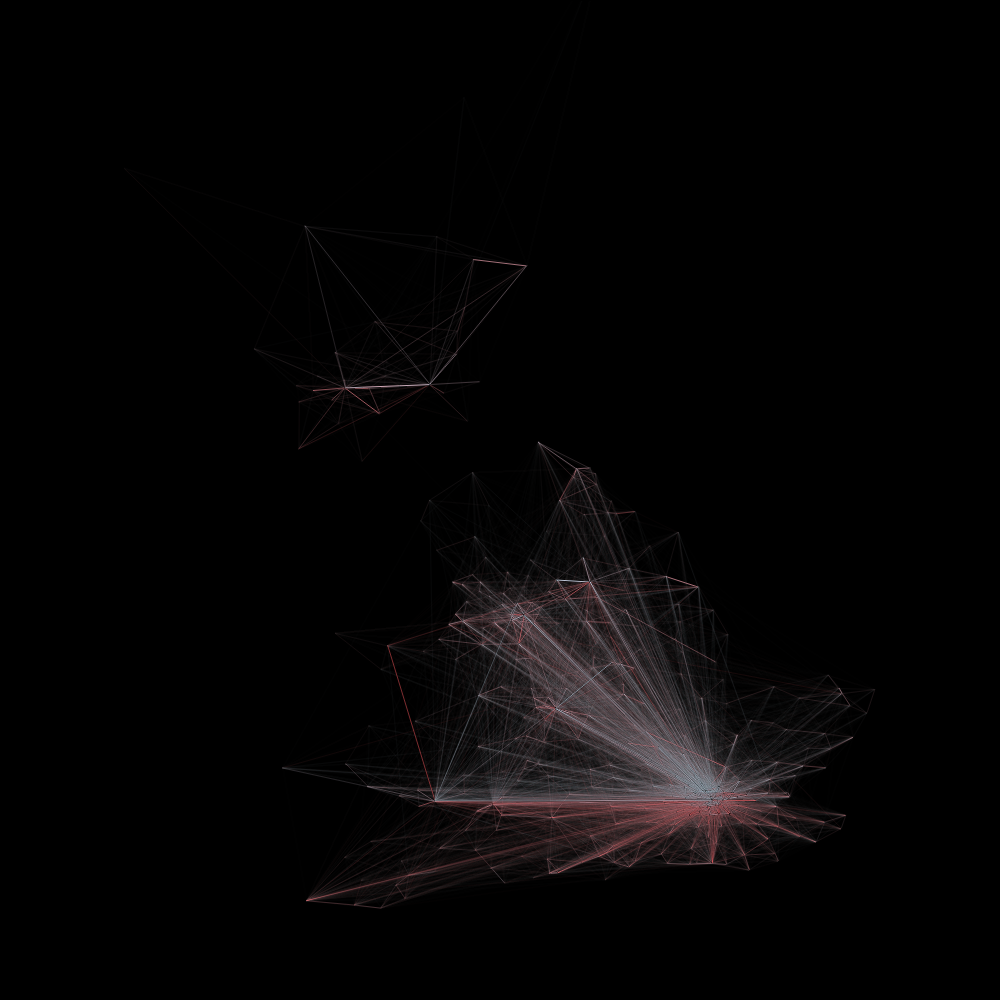
\includegraphics[width=340px]{graphics/visulisation}
 \caption{Visulisation of all company migrations of active companies. Higher opacity means more companies, red line means migration is south to north, black north to south}
\end{figure}

\section{Raw Data}
\subsection{Companies House}
\href{https://www.gov.uk/government/organisations/companies-house}{Companies House} is the database of registered companies\footnote{Need to check definition of a company} in the UK. The database contains the registered address, standard industrial classification (SIC) code, age, number of mortgages, and sometimes turnover information depending on the size of the company. Every month Companies House releases a snapshot of all the active\footnote{According to Companies house records - the company hasn't told companies house that it is inactive.} registered companies. This is the easiest way to get company data, but Companies House does have an open \href{https://developer.companieshouse.gov.uk/api/docs/}{API} which can be used to get more detailed data by processing filing histories of individual companies. This can be used to see the evolution of a set of companies through time. The API has to be used on an individual company basis so to get data for a particular company it's Company ID is required. As the API doesn't have a call to dump a list of company numbers, to use the API the company numbers need to be acquired. Company numbers can be taken from the Companies House snapshots. If looking at aspects of companies through time it may be important to have the company numbers of companies that are no longer active but were active during the time of the sample. \href{https://web.archive.org/web/*/http://download.companieshouse.gov.uk/en_output.html}{Archived} versions of the Companies House snapshot can be used to get company numbers of inactive companies from 2012 and onwards.
\subsection{ONS}
ONS releases fairly detailed business data on a yearly basis. The data broken down by SIC code and location - up to local authority level. The data contains information about enterprises, defined by ONS as `units with a certain level of autonomy', and local units which are parts of an enterprise. For this analysis of the ONS and Companies House data, it is assumed that an enterprise is a collection of Companies House companies. Data before 2014 needs to be accessed through the archive of the old ONS website. ONS also releases data (position, area, name - id look up) on each of the UK's local authorities as well as postcode look up tables to match postcodes to local authorities.

\section{Issues matching Companies House companies to ONS Enterprises}
For the years 2012 - Present, there are about $10^6$ more companies in the Companies House snapshot than are reported on ONS. This means that in order to combine the two datasets there needs to be a way of deciding which companies to include and which to discard.
\subsection{Power Law with number reported by ONS and number of companies registered on Companies House}
\begin{figure}[ht]

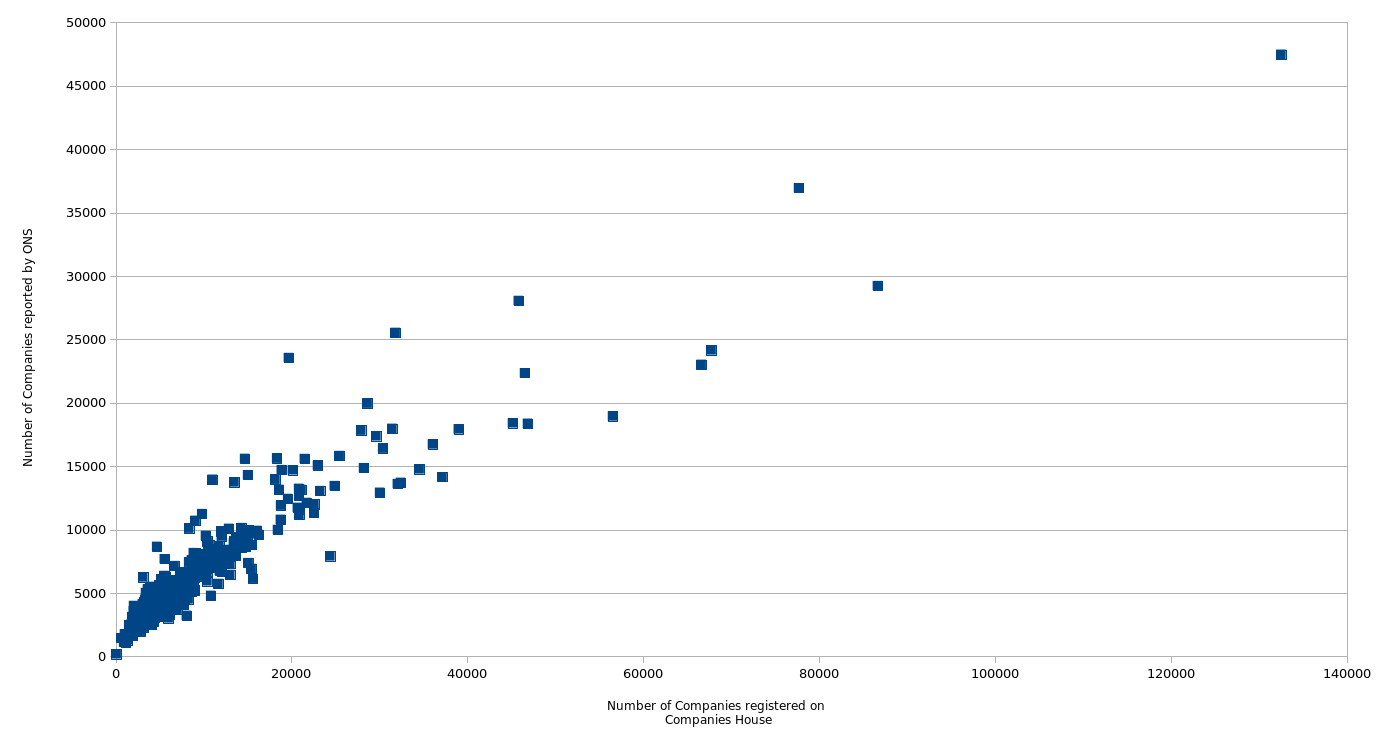
\includegraphics[width=330px]{graphics/2017_ons_against_ch}
\caption{Total companies operating in local authorities against active number registered on Companies House}
\end{figure}




\end{document}
